\documentclass[a4paper,10pt]{article}

\usepackage[english]{babel}
\usepackage{graphicx}
\usepackage[colorlinks, linkcolor=black, citecolor=black, urlcolor=black]{hyperref}
\usepackage{geometry}
\usepackage{ifthen}
\usepackage{booktabs}
\usepackage{array}
\usepackage{caption}
\usepackage{float}
\usepackage{placeins}
\usepackage{amsmath}
\usepackage{amssymb}
\usepackage{microtype}

\geometry{tmargin=1.75cm, bmargin=1.85cm, lmargin=1.65cm, rmargin=1.65cm}
\setlength{\parindent}{0pt}
\setlength{\parskip}{2pt}
\setlength{\textfloatsep}{5pt plus 2pt minus 2pt}
\setlength{\floatsep}{5pt plus 2pt minus 2pt}
\setlength{\intextsep}{5pt plus 2pt minus 2pt}
\captionsetup{font=small, skip=3pt}
\renewcommand{\arraystretch}{1.02}
\raggedbottom
\setcounter{topnumber}{4}
\setcounter{bottomnumber}{2}
\setcounter{totalnumber}{6}
\renewcommand{\topfraction}{0.96}
\renewcommand{\bottomfraction}{0.9}
\renewcommand{\textfraction}{0.03}
\renewcommand{\floatpagefraction}{0.8}

\begin{document}
\newboolean{anonymize}

\begin{titlepage}
    \newpage
    \thispagestyle{empty}
    \frenchspacing
    \hspace{-0.2cm}
    
\includegraphics[height=3.4cm]{assets/sedes.pdf}
    \hspace{0.2cm}
    \rule{0.5pt}{3.4cm}
    \hspace{0.2cm}
    \begin{minipage}[b]{8cm}
        \Large{Katholieke\newline Universiteit\newline Leuven}\smallskip\newline
        \large{}\smallskip\newline
        \textbf{Department of\newline Computer Science}\smallskip
    \end{minipage}
    \hspace{\stretch{1}}
    \vspace*{3.2cm}\vfill
    \begin{center}
        \begin{minipage}[t]{\textwidth}
            \begin{center}
                \LARGE{\rm{\textbf{{A Reverse-Hoops-Playing Robot Arm}}}}\\
                \Large{\rm{Robotics (B-KUL-H02A4A)}}
            \end{center}
        \end{minipage}
    \end{center}
    \vfill
    \hfill\makebox[8.5cm][l]{%
        \vbox to 7cm{\vfill\noindent
            \ifthenelse{\boolean{anonymize}}{%
                {\rm \textbf{Anonymized}}\\
                {\rm Academic year 2025--2026}
            }{%
                {\rm \Large{\textbf{Enmin Lin (r0927480)}}}\\[2mm]
                {\rm Academic year 2025--2026}
            }
        }
    }
\end{titlepage}


\small

\section*{Reverse-Hoops-Playing Robot Arm}

\subsection*{System Overview and Experimental Setup}

The task is simple to state: the ball is thrown at the robot, and the UR10 must move the hoop so that the ball passes through it \cite{projectdesc}. The hard part is that the ball measurements are noisy, the robot has joint limits, and the ball only has \(30\,\mathrm{mm}\) of radial clearance inside the hoop. The system is split into three questions. Where will the ball go? Which future point should the robot try to catch? Can the UR10 move the hoop there without breaking its limits?

The main claim of this report is that the second question matters most. The Kalman filter and the NLP controller are kept fixed in the benchmark. Only the interception-point rule changes. This makes the comparison easy to read: a better prediction model alone is not enough, and a point that looks good geometrically may still be impossible for the robot.

\begin{figure}[H]
    \centering
    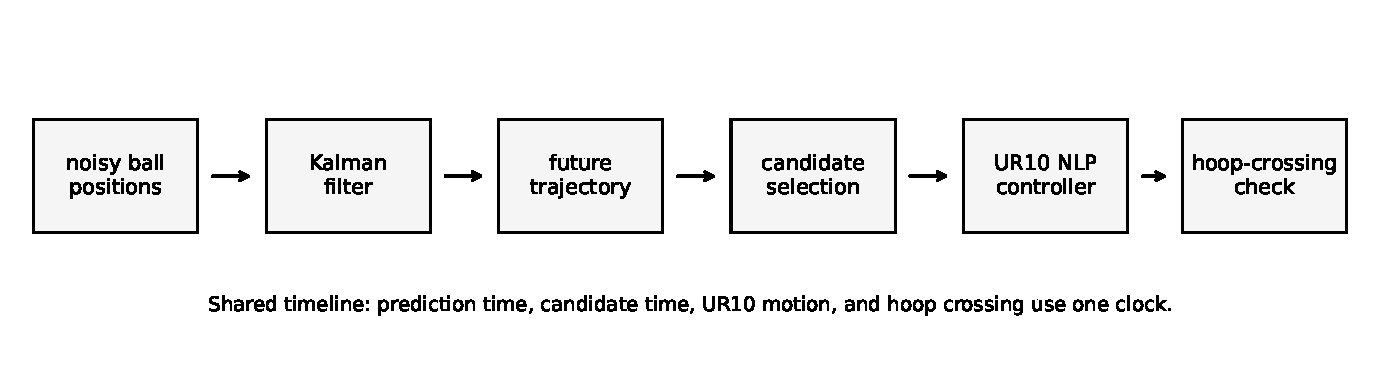
\includegraphics[width=0.95\linewidth]{../outputs/high_score/figure_system_block.pdf}
    \caption{System pipeline used in the benchmark. The same ball prediction, candidate pool, NLP controller, and hoop-crossing metric support all strategy comparisons.}
    \label{fig:system}
\end{figure}

\begin{table}[H]
\centering
\caption{Constants and modelling choices used by the estimator, controller, and success metric.}
\label{tab:assumptions}
\begin{tabular}{@{}p{0.20\linewidth}p{0.27\linewidth}p{0.46\linewidth}@{}}
\toprule
Item & Value & Quantitative role \\
\midrule
Ball and hoop radii & \(0.12,\,0.15\,\mathrm{m}\) & \(r_h-r_b=30\,\mathrm{mm}\) radial tolerance \\
Measurement noise & \(1\,\mathrm{mm}\) Gaussian position noise & \(R=\sigma^2 I_3\) in the Kalman update \\
Robot base & Fixed & Removes mobile-base planning from the report \\
Acceleration limit & \(2\,\mathrm{rad/s^2}\) & \(|\ddot q_{k,j}|\le2\) for every knot and joint \\
Hoop orientation & Top side never faces ground & TCP \(z\)-axis satisfies \(R_{zz}(q_k)\ge0\) \\
Table clearance & Hoop center remains above table & \(z_{\mathrm{tcp}}(q_k)\ge h_{\mathrm{table}}+m_{\mathrm{tcp}}\), hard path constraint \\
Self-collision proxy & Link-sphere clearance check & Positive sphere clearance means no proxy overlap after planning \\
\bottomrule
\end{tabular}
\end{table}

The simulator gives the current robot state and noisy ball positions. Only the ball state is estimated. After a candidate point is chosen, the controller plans one joint trajectory and then executes it open-loop; no MPC is used during the simulation. This is why the benchmark reports two different errors. Terminal TCP error says how well the NLP reaches the predicted target. Radial crossing error says whether the true ball actually passes through the hoop. The simulator includes bounce physics, but every reported catch happens before the first bounce. A post-bounce catch would need a different prediction model.

\subsection*{Task 1: Trajectory Estimation under Position Noise}

The ball state uses position and velocity,
\begin{equation}
x_t=\begin{bmatrix}p_x&p_y&p_z&v_x&v_y&v_z\end{bmatrix}^\top .
\label{eq:kf-state}
\end{equation}
The process model keeps horizontal velocity constant and adds known gravity in \(z\),
\begin{equation}
x_{t+\Delta t}=F x_t+B g+w_t,\qquad y_t=H x_t+v_t,\qquad v_t\sim\mathcal{N}(0,\sigma^2I_3).
\label{eq:kf-model}
\end{equation}
Here \(F\) advances the constant-velocity state, \(Bg\) adds gravity, \(H\) selects the position entries, and \(y_t\) is the measured ball position. Between bounces, this is a linear model. The project also gives Gaussian position noise with known standard deviation.

\emph{Filter choice.} A Kalman filter fits these assumptions directly. The belief is Gaussian, the dynamics are linear, and the measurement model is linear with Gaussian noise. Each step first predicts the mean and covariance, then corrects them with the measurement innovation. Under this model, the Kalman update is the Bayes-optimal MMSE estimate and also gives an analytic covariance \cite{kalman1960}. The covariance is useful because it shows whether prediction uncertainty is small compared with the \(30\,\mathrm{mm}\) hoop clearance. An EKF would reduce to the same update here, and a particle filter would add sampling noise without adding useful modelling power.

The filter starts from the first noisy ball position. Its initial velocity is set to zero, but with a large velocity covariance so that later measurements can quickly correct it. The robot state is available from the simulator, so the estimator only tracks the ball. Across 50 seeds at the project noise level, raw measurement RMSE was \(1.74\,\mathrm{mm}\), filtered RMSE was \(0.90\,\mathrm{mm}\), and 0.5 s future-prediction RMSE was \(3.51\,\mathrm{mm}\). The 95th percentile future-prediction RMSE was \(6.35\,\mathrm{mm}\), still far below the \(30\,\mathrm{mm}\) hoop clearance.

\begin{figure}[H]
    \centering
    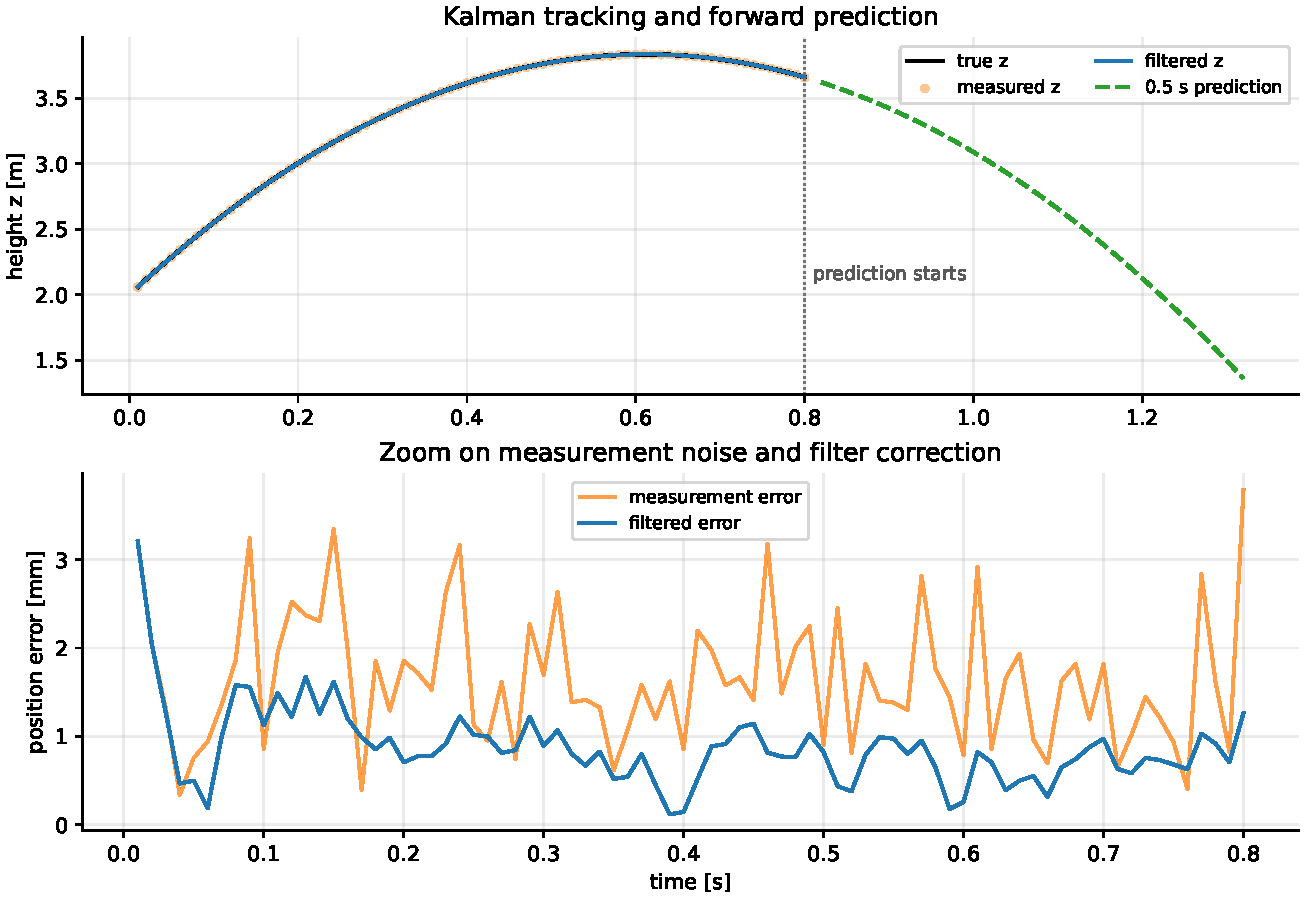
\includegraphics[width=0.88\linewidth]{../outputs/task1/task1_trajectory_prediction.pdf}
    \caption{Kalman-filter prediction for one seed. The lower panel shows that filtering removes most of the 1 mm measurement jitter, and the 50-seed validation keeps the 0.5 s prediction error below \(6.35\,\mathrm{mm}\) at the 95th percentile.}
    \label{fig:task1}
\end{figure}

A noise sweep checks how much this result depends on the exact noise level. When measurement noise increases from 1 to 10 mm, mean 0.5 s prediction RMSE increases from \(3.67\) to \(10.34\,\mathrm{mm}\), and the largest observed RMSE stays at \(20.01\,\mathrm{mm}\). The sweep uses a different seed set, so the small difference between \(3.51\,\mathrm{mm}\) and \(3.67\,\mathrm{mm}\) is just sampling variation. Even at higher noise, the prediction error remains below the \(30\,\mathrm{mm}\) radial clearance. Estimation is not the main bottleneck in this setup.

\subsection*{Task 2: Geometric Candidate Selection Baselines}

Task 2 only asks for a simple interception point. The baseline therefore does not solve a robot motion problem yet. It samples the predicted ball trajectory and rejects points that are too soon, too low, or too far from the current hoop center. The standalone Task 2 validation uses a \(0.85\,\mathrm{m}\) workspace radius. We use this coarse workspace-radius filter as a simple reachability proxy, and the later Task 3 tests confirm that this proxy is conservative. The Task 4 benchmark uses a wider \(1.15\,\mathrm{m}\) radius so that all strategies start from the same larger candidate pool. With that wider pool, the simple rule tries earlier points, so its 50-seed mean attempt time is \(1.295\,\mathrm{s}\), earlier than the standalone \(1.36\,\mathrm{s}\) pick. For the validation seed, the rule selected \([1.224,-0.119,1.074]\,\mathrm{m}\).

This rule answers only one question: where does the ball pass through a reasonable region of space? It does not check whether the UR10 can move the hoop there with the right pose and acceleration. Across 50 seeds, the simple geometric rule attempted an early catch at \(1.295\pm0.012\,\mathrm{s}\), but it produced 0 successful catches under the full NLP and hoop-crossing check.

A second baseline removes prediction completely. It uses a damped Jacobian pseudo-inverse Cartesian velocity controller,
\begin{equation}
\dot q = J(q)^\top\left(J(q)J(q)^\top+\lambda^2I\right)^{-1}K(p_{\mathrm{ball,meas}}-p_{\mathrm{tcp}}),
\label{eq:reactive}
\end{equation}
with proportional gain \(K\), damping \(\lambda\), and velocity and acceleration saturation. This reactive controller also gives 0\% success. Its closest TCP-to-ball distance was \(0.176\pm0.058\,\mathrm{m}\), and even the best seed stayed \(59.4\,\mathrm{mm}\) away, about twice the \(30\,\mathrm{mm}\) radial tolerance. It can chase the ball, but it cannot arrive at the right place at the right time. Prediction is necessary, and a predicted point by itself is still not enough.

\begin{figure}[H]
    \centering
    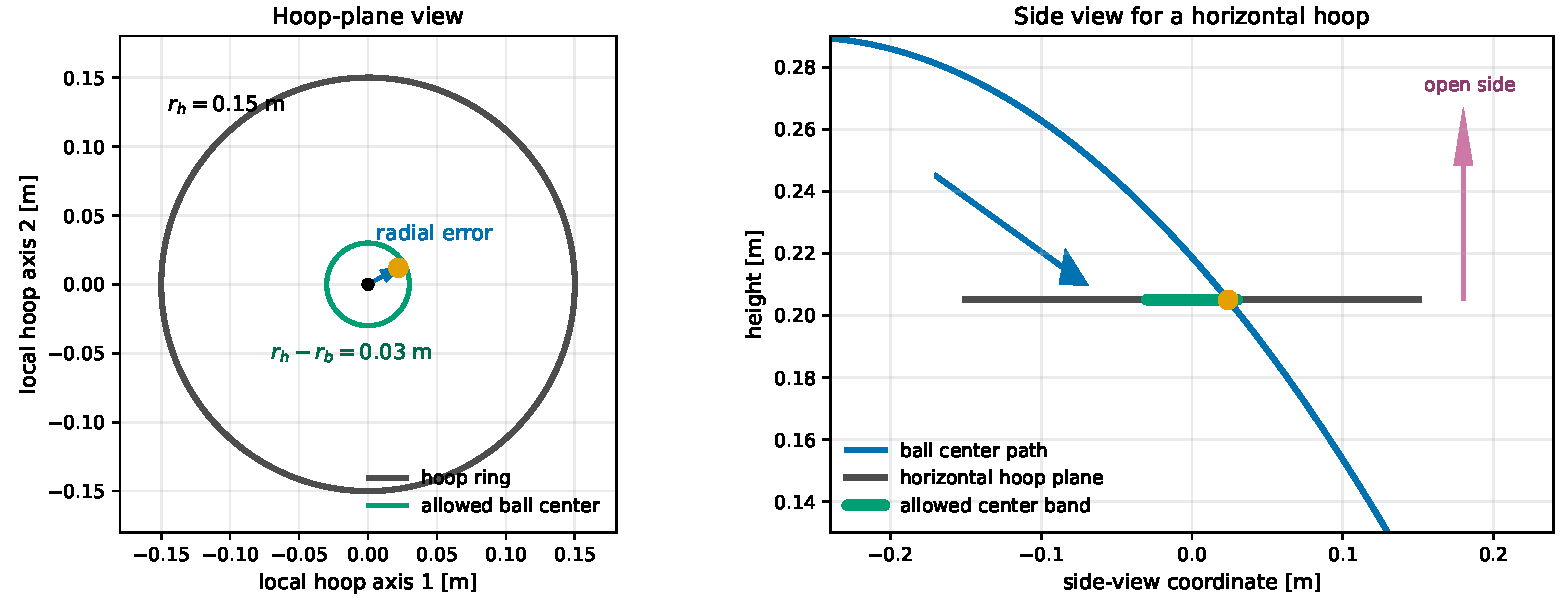
\includegraphics[width=0.86\linewidth]{../outputs/high_score/figure_hoop_geometry_definition.pdf}
    \caption{Success metric used in Task 3 and Task 4. The ball center must cross the hoop plane and lie within the \(r_h-r_b=30\,\mathrm{mm}\) radial band; otherwise the ball touches the ring or misses the opening.}
    \label{fig:geometry}
\end{figure}

\subsection*{Task 3: Constrained Trajectory Optimization for the UR10}

The controller plans the robot motion with a finite-horizon nonlinear program. The decision variables are joint position, velocity, and acceleration,
\begin{equation}
\{q_k,\dot q_k\}_{k=0}^{N},\quad \{\ddot q_k\}_{k=0}^{N-1}.
\label{eq:decision-vars}
\end{equation}
The plan must obey the second-order joint dynamics
\begin{equation}
q_{k+1}=q_k+\dot q_k\Delta t+\tfrac{1}{2}\ddot q_k\Delta t^2,\qquad
\dot q_{k+1}=\dot q_k+\ddot q_k\Delta t .
\label{eq:dynamics}
\end{equation}
The optimization problem is
\begin{equation}
\begin{aligned}
\min_{q,\dot q,\ddot q}\;&
w_p\|p_{\mathrm{tcp}}(q_N)-p^\star\|_2^2
+\sum_{k=0}^{N-1} w_u\|\ddot q_k\|_2^2
+\sum_{k=1}^{N} w_v\|\dot q_k\|_2^2\\
&+w_o(1-R_{zz}(q_N))^2
+w_n\bigl(1-(n_{\mathrm{hoop}}(q_N)^\top\hat v_{\mathrm{ball}})^2\bigr)\\
\mathrm{s.t.}\;& q_0=q_{\mathrm{init}},\quad \dot q_0=\dot q_{\mathrm{init}},\\
& q_{\min}\le q_k\le q_{\max},\quad
-\dot q_{\max}\le \dot q_k\le \dot q_{\max},\quad
-\ddot q_{\max}\le \ddot q_k\le \ddot q_{\max},\\
& z_{\mathrm{tcp}}(q_k)\ge h_{\mathrm{table}}+m_{\mathrm{tcp}},\quad
R_{zz}(q_k)\ge0,\qquad \forall k .
\end{aligned}
\label{eq:nlp}
\end{equation}
Equation~\ref{eq:dynamics} prevents the optimizer from jumping between unrelated joint states. In Eq.~\ref{eq:nlp}, \(p^\star\) is the predicted ball position at the catch time, \(p_{\mathrm{tcp}}\) is the hoop-center position, \(n_{\mathrm{hoop}}\) is the hoop normal, and \(\hat v_{\mathrm{ball}}\) is the unit ball velocity at the catch point. The first cost term moves the hoop center to the ball. The next two terms keep acceleration and velocity small. The last two terms keep the hoop upright and align the hoop with the ball direction. The squared dot product treats the two normal directions symmetrically, while the hard \(R_{zz}\ge0\) path constraint keeps the upright branch. The inequalities enforce joint position, velocity, acceleration, table-clearance, and top-side orientation limits.

The validation uses \(N=28\), \(\Delta t=0.05\,\mathrm{s}\), \(w_p=1500\), \(w_u=2\times10^{-2}\), \(w_v=10^{-3}\), \(w_o=10\), and \(w_n=5\). This gives a \(1.4\,\mathrm{s}\) validation horizon. In the benchmark, the horizon is recomputed for each candidate catch time. In the URDF, the fixed tool-to-TCP transform maps the physical ring normal to the TCP \(z\)-axis. The controller therefore uses TCP \(z\) as \(n_{\mathrm{hoop}}\). The scalar \(R_{zz}=e_z^\top R_{\mathrm{tcp}}(q)e_z\) is the world-\(z\) component of that axis. The constraint \(R_{zz}(q_k)\ge0\) keeps the top side from pointing below the horizontal plane. Pinocchio supplies URDF forward kinematics \cite{carpentier2019}. CasADi builds the symbolic NLP \cite{andersson2019}, and IPOPT solves it \cite{wachter2006}.

\begin{figure}[H]
    \centering
    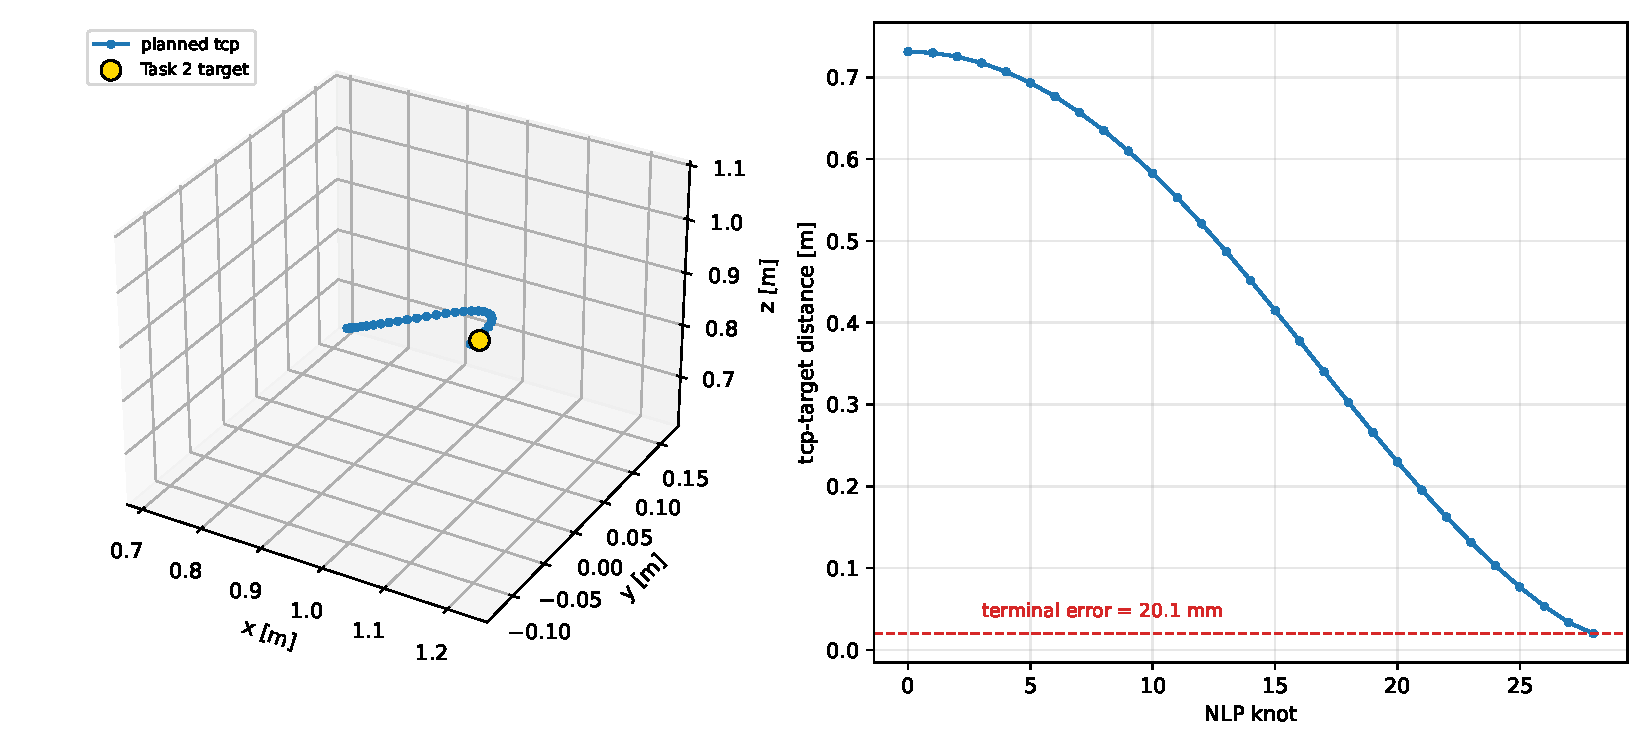
\includegraphics[width=0.82\linewidth]{../outputs/task3/task3_layer1_plan.pdf}
    \caption{Task 3 finite-horizon NLP result. The hoop center reaches \(20.1\,\mathrm{mm}\) terminal TCP error while the path constraints keep the motion executable.}
    \label{fig:task3}
\end{figure}

\begin{figure}[H]
    \centering
    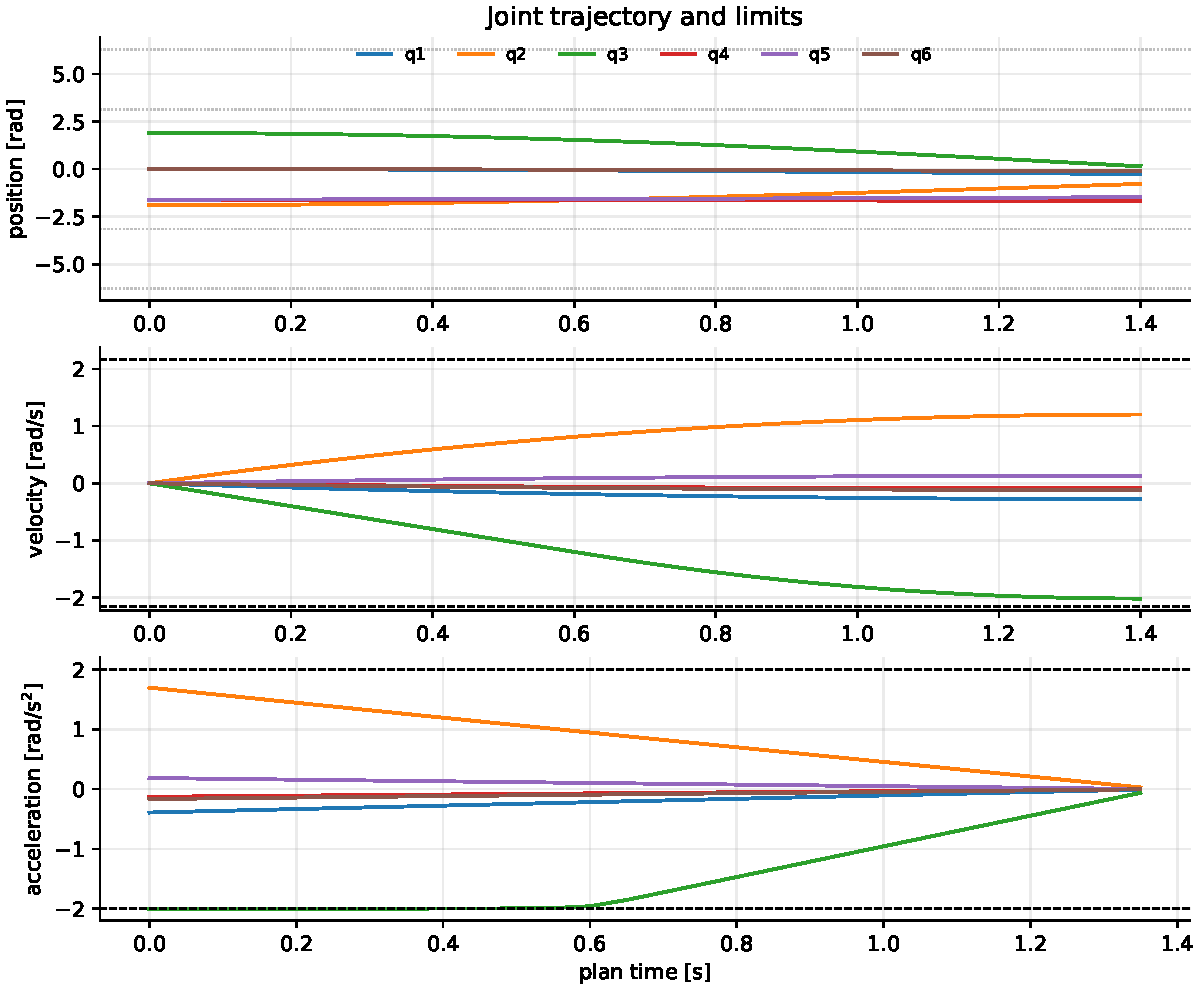
\includegraphics[width=0.82\linewidth]{../outputs/task3/task3_joint_limits.pdf}
    \caption{Joint profiles for the same plan. All accelerations approach but do not exceed \(\pm2\,\mathrm{rad/s^2}\), and joint 2 reaches the highest velocity utilization at 64\% of its limit.}
    \label{fig:joints}
\end{figure}

Figure~\ref{fig:task3} shows what the NLP does in space: the hoop center moves from a large initial offset to a \(20.1\,\mathrm{mm}\) terminal error at the selected catch point. Figure~\ref{fig:joints} shows why the motion is difficult. The robot is not mainly limited by velocity; joint 2 uses only 64\% of its velocity bound. The tight limit is acceleration, because the acceleration profile touches the \(\pm2\,\mathrm{rad/s^2}\) bound.

For the Task 2 target, the NLP reduced the hoop-target distance from \(0.731\,\mathrm{m}\) to \(0.020\,\mathrm{m}\). It solved in \(0.071\,\mathrm{s}\) and 15 IPOPT iterations on the validation run. The maximum acceleration was \(1.9996\,\mathrm{rad/s^2}\), the maximum velocity ratio was 0.640, and the minimum \(R_{zz}\) value was 0.732. The minimum TCP-table clearance was \(0.622\,\mathrm{m}\), the minimum frame-table clearance was \(0.115\,\mathrm{m}\), and the minimum self-collision clearance proxy was \(0.163\,\mathrm{m}\). Table clearance and hoop orientation are hard NLP path constraints. Self-collision is checked after planning with a conservative link-sphere proxy, not with exact mesh distances.

This result should be read as a controller validation. Task 3 shows that the UR10 can move the hoop center close to the predicted target. Final catch success still depends on where the true ball crosses the hoop plane, so the full catch check is evaluated in Task 4.

Exact mesh self-collision would add many non-smooth distance constraints. For this report, all successful plans are required to keep positive clearance under the sphere proxy. A stricter version could add capsule or sphere signed-distance constraints directly to Eq.~\ref{eq:nlp}.

The \(w_o\) ablation checks whether the upright-orientation soft cost is doing the main work. It is not. Across \(w_o\in\{0,1,10,50\}\), time-first benchmark success stayed at 98\%. The hard \(R_{zz}\ge0\) path constraint and the normal-alignment term set the final geometry. The terminal \(R_{zz}\) cost mainly regularizes the pose.

\subsection*{Task 4: Feasibility-Aware Candidate Selection}

Task 4 asks for a smarter interception point with higher success rate and shorter interception time. The submitted strategy is the time-first feasible selector. It chooses the earliest candidate that passes the predicted-candidate, NLP-feasibility, and safety checks. The selector is computed from predicted candidates, NLP feasibility, and safety metrics. The true-ball hoop-crossing check is used as the benchmark success metric after selection. The balanced and late-feasible selectors are kept as comparison cases, because they show what is gained by waiting longer.

The simple geometric rule tries an earlier catch, but it has 0\% success. Its time is therefore only an attempted time, not a successful catch time. For a fair comparison, all policies are evaluated on the same candidate pool. The selector samples the predicted trajectory and solves the Task 3 NLP for each shortlisted candidate. A benchmark attempt is counted as successful only if the NLP converges, the true ball crosses the hoop plane inside the tolerance, and the safety penalty is zero. All 396 evaluated candidate NLPs converged, but only 164 candidate attempts passed the hoop-crossing test. On average, each seed had \(7.9\) evaluated candidates and \(3.3\) benchmark-successful catches. About 59\% of geometrically plausible candidates were rejected after the full check. This is the main bottleneck: the robot can often solve the motion plan, but many candidate times do not put the hoop in the right crossing geometry. Compared with the simple geometric attempt at \(1.295\,\mathrm{s}\), the time-first feasible selector catches \(92\,\mathrm{ms}\) later. That number is catch-time delay, not computation time. The delay is about two control ticks because the NLP uses \(\Delta t=50\,\mathrm{ms}\), and it raises success from 0\% to 98\%.

The balanced selector ranks feasible candidates by catch time, terminal TCP error, acceleration use, velocity use, and safety penalty, with weights \(15.0,100.0,0.20,0.20,50.0\). The time-first and late-feasible policies use the same candidate pool but select the earliest or latest successful candidate. Figure~\ref{fig:side} shows the difference visually: red marks the simple geometric pick, and yellow marks the feasible catch that the UR10 can actually make.

Two extra checks point to the same conclusion. The bottleneck is geometric feasibility, not estimator quality. In a 1--10 mm noise sweep over 20 downstream seeds, time-first success stayed at 95\% for every tested noise level. With 20 seeds, one failure changes the rate by 5\%, so this matches the 50-seed 98\% result. A covariance-rejection ablation also selected the same catches as time-first feasible across all 50 seeds when it removed candidates above a conservative \(0.18\,\mathrm{m}\) forward-covariance threshold. The covariance is useful for diagnosis, but it is not the deciding signal in this open-loop benchmark.

\begin{figure}[H]
    \centering
    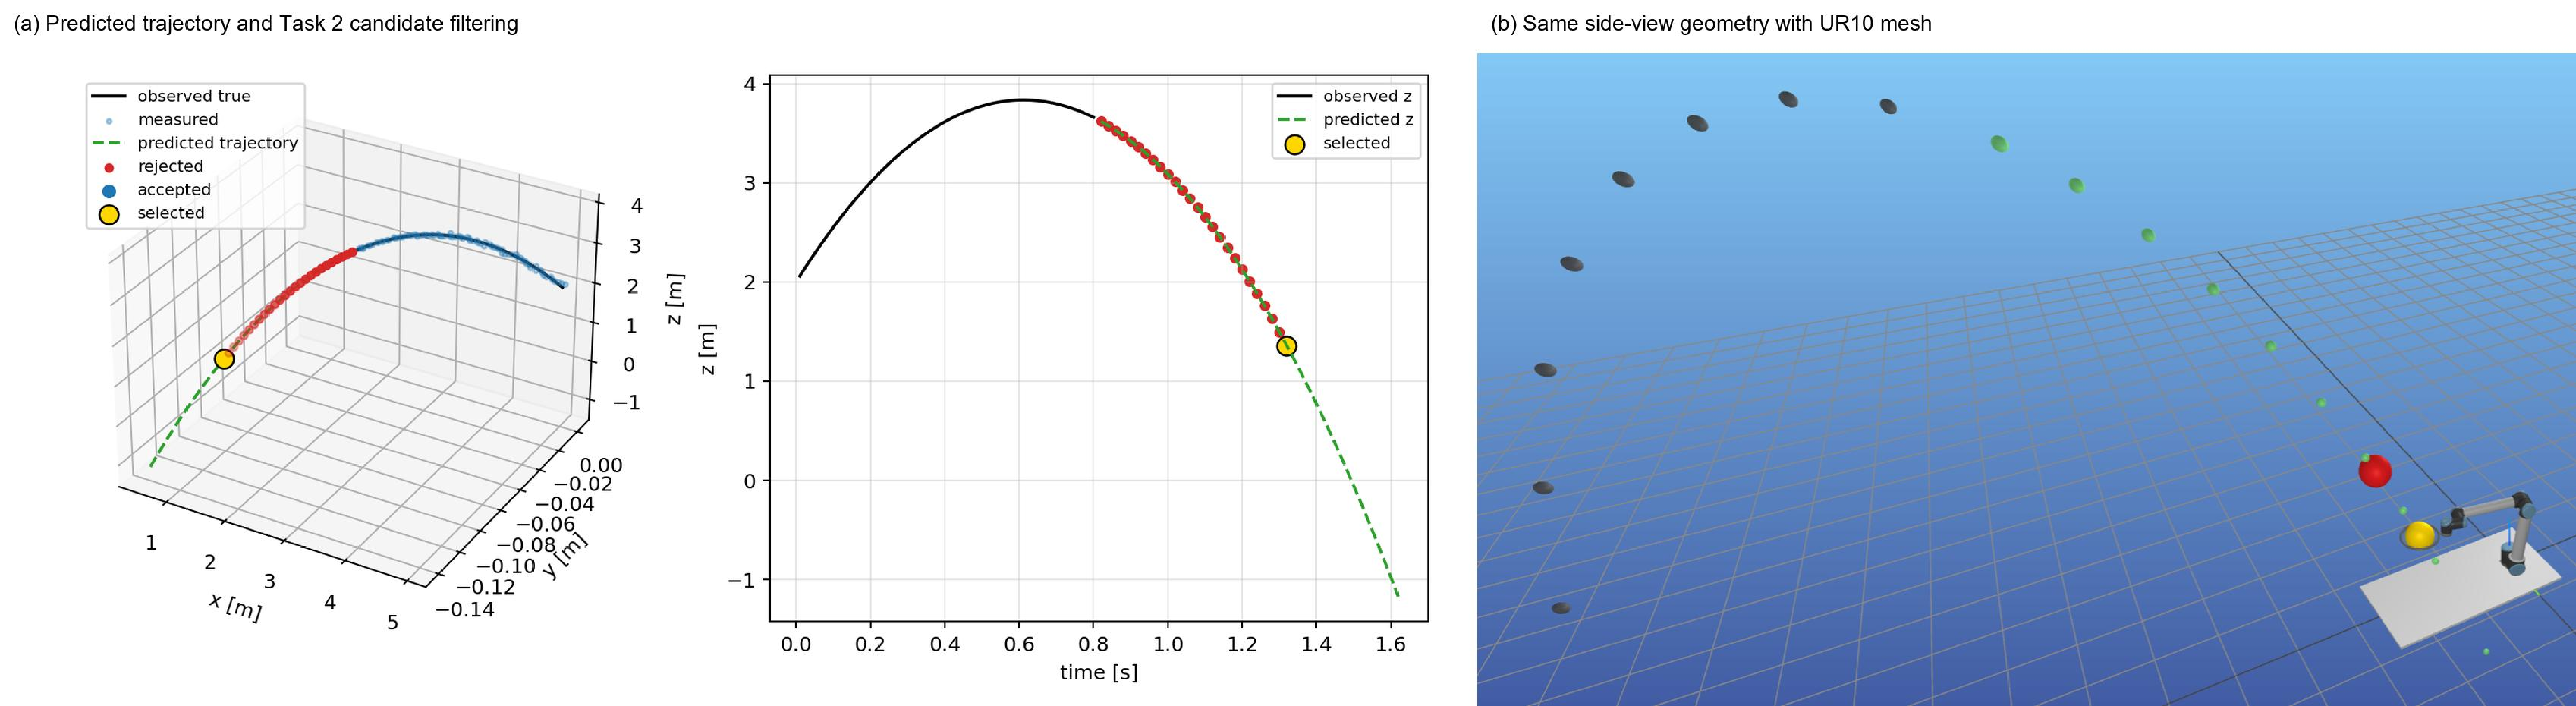
\includegraphics[width=0.92\linewidth]{../outputs/high_score/figure_task2_task4_side_by_side.pdf}
    \caption{Task 2 and Task 4 candidate geometry in matching views. The left panels show predicted-trajectory filtering for the candidate pool; the right panel renders the same scene in Meshcat. Colors: grey = observed past trajectory, green = predicted future trajectory, red = simple geometric candidate, yellow = selected feasible catch.}
    \label{fig:side}
\end{figure}

\begin{figure}[H]
    \centering
    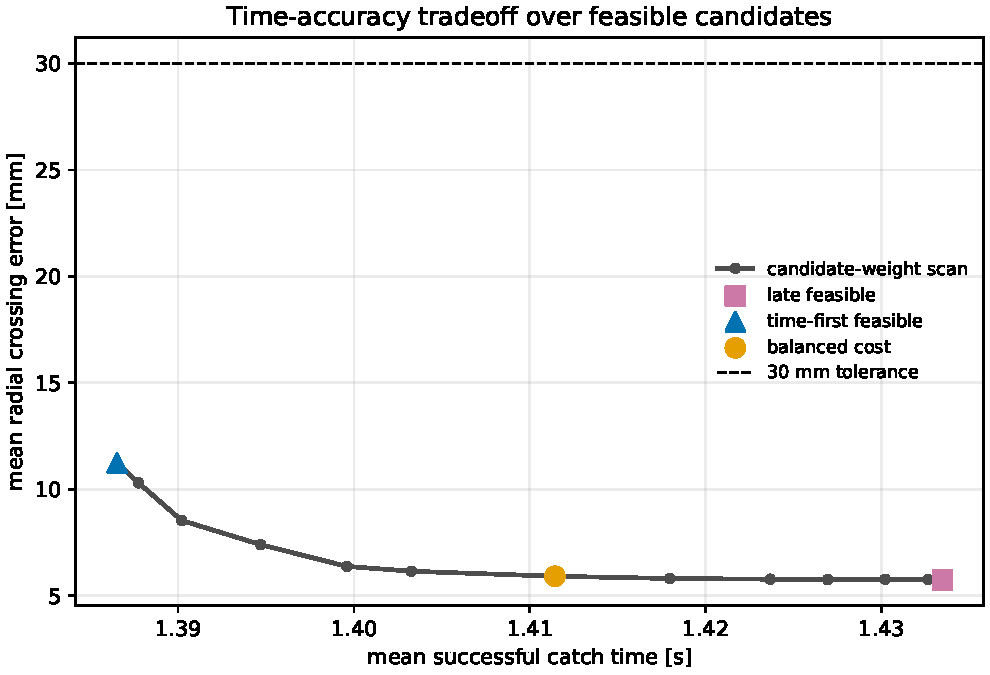
\includegraphics[width=0.72\linewidth]{../outputs/high_score/figure_candidate_pareto.pdf}
    \caption{Empirical candidate-weight scan on the time-accuracy plane. Time-first gives the early-time end, late feasible gives the accurate but slower end, and the elbow near balanced cost buys roughly \(5\,\mathrm{mm}\) of radial accuracy for about \(25\,\mathrm{ms}\).}
    \label{fig:pareto}
\end{figure}

\begin{table}[H]
\centering
\caption{Final 50-seed benchmark. Time is catch time from ball release. TCP is terminal hoop-center error to the predicted target. Radial is true hoop-plane crossing error. Max \(\ddot q\) is the largest absolute joint acceleration in \(\mathrm{rad/s^2}\), with hard bound 2. The asterisked simple time is attempted, not successful.}
\label{tab:summary}
\begin{tabular}{@{}lcccccc@{}}
\toprule
Strategy & Success & Time [s] & TCP [mm] & Radial [mm] & Max \(\ddot q\) & IPOPT \\
\midrule
Reactive no prediction & 0\% & -- & -- & -- & -- & -- \\
Simple geometric & 0\% & 1.295* & -- & -- & -- & -- \\
Late feasible & 98\% & \(1.433\pm0.009\) & 1.87 & 5.75 & 1.65 & 10.4 it. \\
Time-first feasible & 98\% & \(1.387\pm0.018\) & 13.18 & 11.24 & 2.00 & 13.5 it. \\
Balanced cost & 98\% & \(1.411\pm0.015\) & 3.22 & 5.91 & 1.81 & 12.3 it. \\
\bottomrule
\end{tabular}
\end{table}
The time-first feasible policy is the clearest answer to Task 4. It raises full-system success from 0\% to 98\%. Among the successful feasible policies, it catches \(0.025\,\mathrm{s}\) earlier than balanced cost and \(0.047\,\mathrm{s}\) earlier than late feasible. The larger gap is about one control tick. Late feasible is more accurate, and balanced cost sits between the two. The report uses time-first as the Task 4 strategy because the task asks for shorter interception time. If the goal were best radial accuracy instead, balanced cost or late feasible would be the better engineering choice. Figure~\ref{fig:pareto} shows this time-accuracy tradeoff directly.

Time-first runs with the tightest motion budget. The NLP often hits the acceleration bound, so it has less room to refine the final pose. Balanced and late-feasible candidates happen later, where the robot has more time to align the hoop with the ball direction. That is why those rows have lower TCP and radial errors. The TCP column is the hoop-center error at the NLP terminal knot. The radial column is the hoop-to-ball error when the true ball crosses the hoop plane. These are different checks. With time-first, the hoop can sweep past the ball, so the crossing instant can be closer than the terminal knot. Late feasible drives TCP error below \(2\,\mathrm{mm}\). Its radial error stays near \(6\,\mathrm{mm}\) because the true ball crosses a few millimetres away from the predicted target.

The open-loop gap is small in the successful time-first catches. The NLP terminal error to the predicted target averaged \(13.18\,\mathrm{mm}\). The predicted hoop-crossing radial error averaged \(9.36\,\mathrm{mm}\), while the true-ball radial error averaged \(11.24\,\mathrm{mm}\). The means differ by \(1.87\,\mathrm{mm}\), and the per-seed mean absolute predicted-to-true radial gap is \(4.41\,\mathrm{mm}\). This keeps solver error and execution error separate.

\subsection*{Failure Analysis and Interpretation}

The only time-first failure is seed 11. Figure~\ref{fig:failure} shows why it is difficult: this throw is near the 95th percentile of the 50-seed lateral velocity distribution. After the hoop normal was fixed to the TCP \(z\)-axis in the Task 3 setup, seed 11's best radial error dropped from \(145.2\) to \(51.5\,\mathrm{mm}\). That is a large improvement, but it still misses the \(30\,\mathrm{mm}\) tolerance. The same correction recovered seed 41, which now crosses at \(24.7\,\mathrm{mm}\).

The seven shortlisted seed 11 candidates all solve the NLP and all cross the hoop plane. None crosses inside the radial tolerance. Their radial errors fall from \(758\) to \(51.5\,\mathrm{mm}\) as catch time moves from \(1.32\) to \(1.44\,\mathrm{s}\). The \(758\,\mathrm{mm}\) case is the earliest candidate, where the UR10 cannot reach the target in time. Every candidate reaches the \(2\,\mathrm{rad/s^2}\) acceleration bound. Early candidates saturate joint 3, and later candidates saturate joint 2. This is an acceleration-limited geometry failure, not a failed estimator or a failed NLP solve.

A mitigation run with 16 candidates and a \(1.35\,\mathrm{m}\) workspace radius did not recover seed 11. The default setting uses 8 candidates and a \(1.0\,\mathrm{m}\) radius. Recovering this seed would likely require a longer prediction horizon or a different candidate sampler.

\begin{figure}[H]
    \centering
    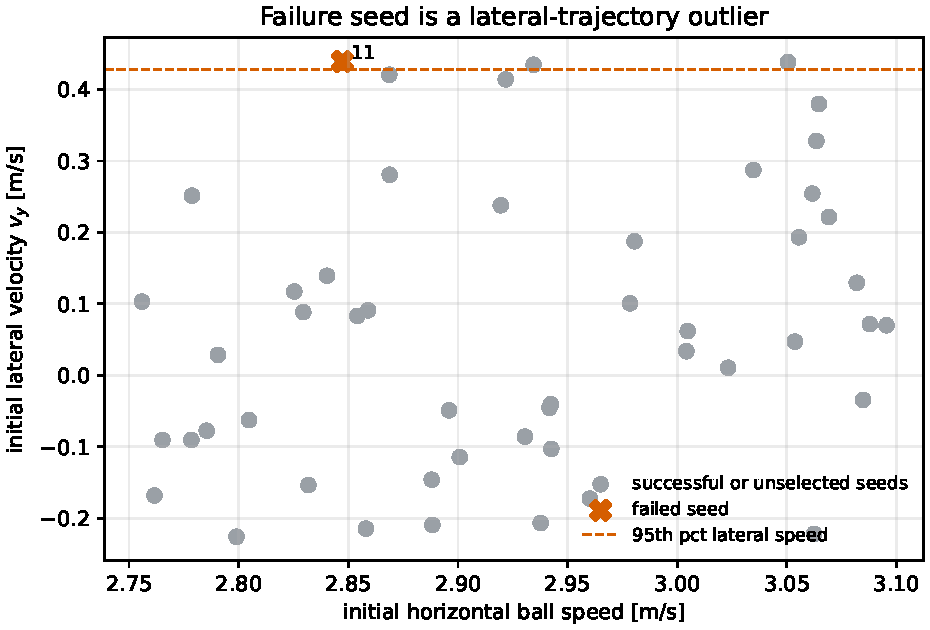
\includegraphics[width=0.58\linewidth]{../outputs/high_score/figure_failure_velocity_diagnostics.pdf}
    \caption{Failure mechanism for seed 11. The red marker is the failed seed and the grey markers are the other seeds; the dashed line marks the empirical 95th percentile of lateral velocity. Seed 11 sits near this high-\(v_y\) boundary and fails by acceleration-limited geometry, not estimator divergence or NLP failure.}
    \label{fig:failure}
\end{figure}

The final architecture uses direct-transcription optimal control with hard physical constraints and soft secondary objectives. This choice is necessary here. A single-step Jacobian controller can chase a Cartesian target, but it cannot save acceleration for a future catch. A closed-form smooth trajectory can reduce jerk, but it does not enforce hoop crossing, joint limits, and top-side orientation together. The horizon NLP is the smallest formulation in this report that handles all of these requirements at once.

\subsection*{Conclusion}

The experiments support the claim made at the start. Prediction is necessary: the reactive controller never reaches the ball within the tolerance. Prediction alone is not enough: the simple geometric selector also gives 0\% success. The decisive step is feasibility-aware candidate selection. It keeps the estimator and controller fixed, filters candidates through the UR10 NLP and the true hoop-crossing check, and raises success to 98\%. Time-first feasible gives the shortest successful catch among the tested policies. Balanced cost shows what it costs, in time, to buy a few extra millimetres of radial accuracy.

\clearpage
\begin{thebibliography}{9}
    \bibitem{projectdesc} Robotics course project description, \emph{A Reverse-Hoops-Playing Robot Arm}, KU Leuven, 2025--2026.
    \bibitem{kalman1960} R. E. Kalman, ``A New Approach to Linear Filtering and Prediction Problems,'' \emph{Journal of Basic Engineering}, 82(1), 35--45, 1960. DOI: 10.1115/1.3662552.
    \bibitem{wachter2006} A. W\"achter and L. T. Biegler, ``On the implementation of an interior-point filter line-search algorithm for large-scale nonlinear programming,'' \emph{Mathematical Programming}, 106, 25--57, 2006. DOI: 10.1007/s10107-004-0559-y.
    \bibitem{andersson2019} J. A. E. Andersson, J. Gillis, G. Horn, J. B. Rawlings, and M. Diehl, ``CasADi: a software framework for nonlinear optimization and optimal control,'' \emph{Mathematical Programming Computation}, 11, 1--36, 2019. DOI: 10.1007/s12532-018-0139-4.
    \bibitem{carpentier2019} J. Carpentier et al., ``The Pinocchio C++ library: a fast and flexible implementation of rigid body dynamics algorithms and their analytical derivatives,'' IEEE/SICE International Symposium on System Integration, 2019.
\end{thebibliography}

\end{document}
